\documentclass[10pt]{article}
% -------------------------------------------------------------------
% Pacotes básicos
\usepackage[english]{babel}										% Idioma a ser usado
                                                                % Trocar "english" para "brazil" para artigos escritos em língua portuguesa 
\usepackage[utf8]{inputenc}										% Escrita de caracteres acentuados e cedilhas - 1
\usepackage[T1]{fontenc}										% Escrita de caracteres acentuados + outros detalhes técnicos fundamentais
% -------------------------------------------------------------------
% Pacotes matemáticos
\usepackage{amsmath,amsfonts,amssymb,amsthm,cancel,siunitx,
calculator,calc,mathtools,empheq,latexsym}
% -------------------------------------------------------------------
% Pacotes para inserção de figuras e subfiguras
\usepackage{subfig,epsfig,tikz,float}		            % Packages de figuras. 
% -------------------------------------------------------------------
% Pacotes para inserção de tabelas
\usepackage{booktabs,multicol,multirow,tabularx,array}          % Packages para tabela
% -------------------------------------------------------------------
\usepackage{float}
\usepackage{biblatex}
\usepackage{hyperref}
% -------------------------------------------------------------------
% Definição de comprimentos
\setlength{\parskip}{5pt}
\textwidth 13.5cm
\textheight 19.5cm
\columnsep .5cm
% -------------------------------------------------------------------
% Título do seu artigo 
\title{\renewcommand{\baselinestretch}{1.17}\normalsize\bf%
\uppercase{Embedded Chessboard Recognition with Convolutional Neural Networks}
}
% -------------------------------------------------------------------
% Autorias
\author{%
José Almeida
}
% -------------------------------------------------------------------

%Início do documento

\begin{document}

\date{}

\maketitle

\vspace{-0.5cm}

\begin{center}
{\footnotesize 
HAW Hamburg, Dept. for Computer Science \\
}
\end{center}

% -------------------------------------------------------------------
% Abstract
\bigskip
\noindent
{\small{\bf ABSTRACT.}
Application of image preprocessing and convolutional neural networks on embedded/mobile (Android) devices for picture recognition of entire chessboards. TensorFlow and Keras are used to fit the model. An Android application was developed to allow for mobile usage of the neural network.
}

\medskip
\noindent
{\small{\bf Keywords}{:} 
computer vision, tensorflow, keras, classification, android, cnn, convolutional neural network, machine learning, opencv
}

\baselineskip=\normalbaselineskip
% -------------------------------------------------------------------

\section{Introduction}\label{sec:1}

More and more technologies are becoming purely digital, but their development may sometimes be hindered because of a necessity to connect them to the real, physical world. Computer vision is one of the main tools making the bridge between both worlds.

The aim of this work is to provide a proof-of-concept foundation for computer vision in relation to board games. In the past, the problem of digitally reading a chessboard has been solved by providing the player with special hardware - like electronic chessboards.

This work tries to solve the problem without using any kind of dedicated hardware, being capable of digitally displaying the complete board state using a picture taken from, for example, a smartphone. This digital representation of the board might then be used in a plethora of ways to improve user/player experience.

\pagebreak

\section{Approach and Architecture}\label{sec:2}

To solve the above layed out problem, it was decided that a convolutional neural network to identify the chess pieces would be used. The training of this neural network, which was made possible by the usage of Keras and TensorFlow, required a dataset, which was partially found on the Internet and partially taken and labeled specifically for this research. After training the network, it is converted into TensorFlow Lite to allow for usage on an Android smartphone.

A PoC/test app was also developed, which allows for taking a picture of the board. The app then preprocesses the image locally, with the help of the OpenCV library, and then queries the TFLite model for every board square, to identify if there is a piece there, and which piece it is. With the result of those queries, the app builds and displays the digital chessboard on the smartphone screen.

\section{Image Preprocessing}\label{sec:3}

The goal of the image preprocessing section is to, given an image, process it in order to separate the chessboard squares, obtaining ROIs, which would be inputs of the neural network model.

The preprocessing of the captured images is perhaps the aspect that required the most time and research to accomplish. All the processing was achieved using the OpenCV library directly. The complete process will be described below.

\begin{figure}[H]
	\centering
	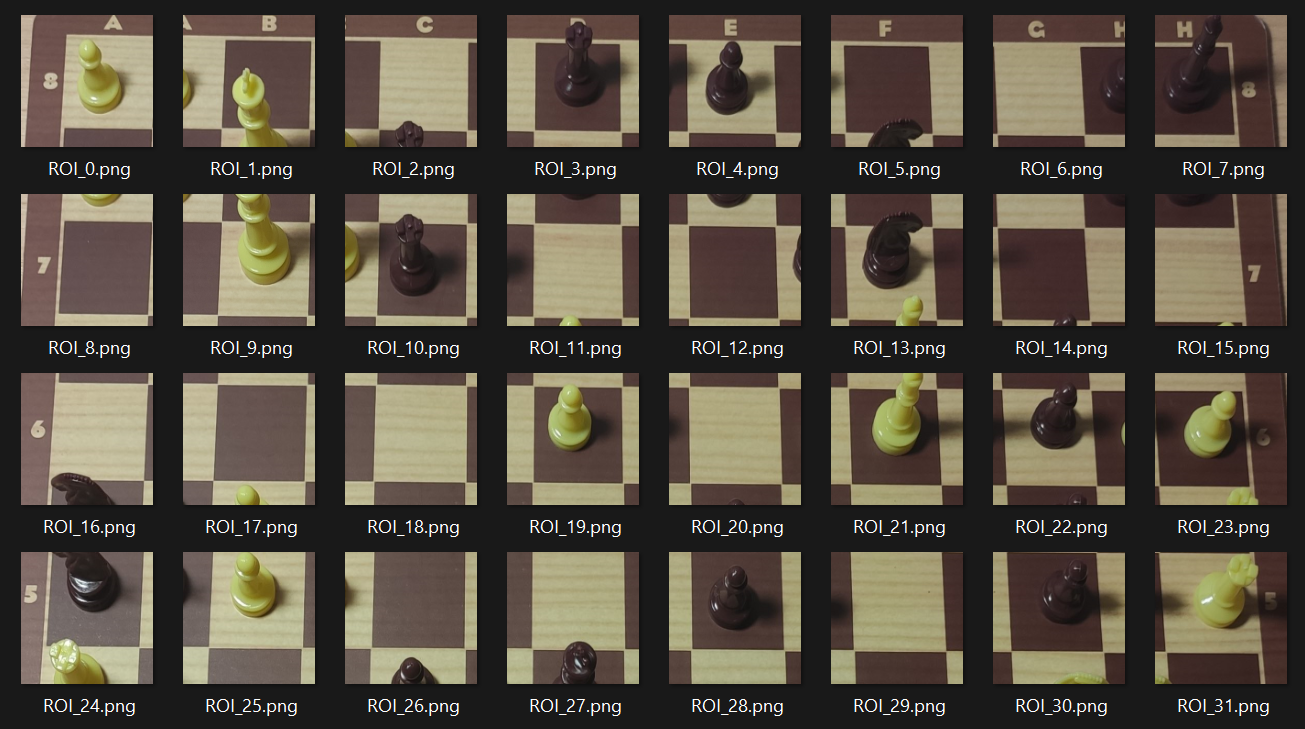
\includegraphics[scale=0.4]{preprocessing-goal}
	\caption{Goal of the image preprocessing.}\label{fig:preprocessing-goal}
\end{figure}

\subsection{Color Space Conversion}

The first step in the preprocessing chain is the conversion of the color space. In this case, the image is converted into a gray color space, so smaller, two-dimensional kernels can be used, which slightly increase efficiency during the image processing.

\subsection{Gaussian Blur}

After the image's color space is converted, a gaussian blur is then applied, which aims to reduce the amount of noise and remove speckles within the image, so as to make any specific image features more recognizable to the CNN. This is done by applying a 2D filter with the same number of columns and rows as the desired image. Each of the matrix element equals, in this case, $\frac{1}{25}$, which is the level of applied Gaussian blur.

\begin{figure}[H]
	\centering
	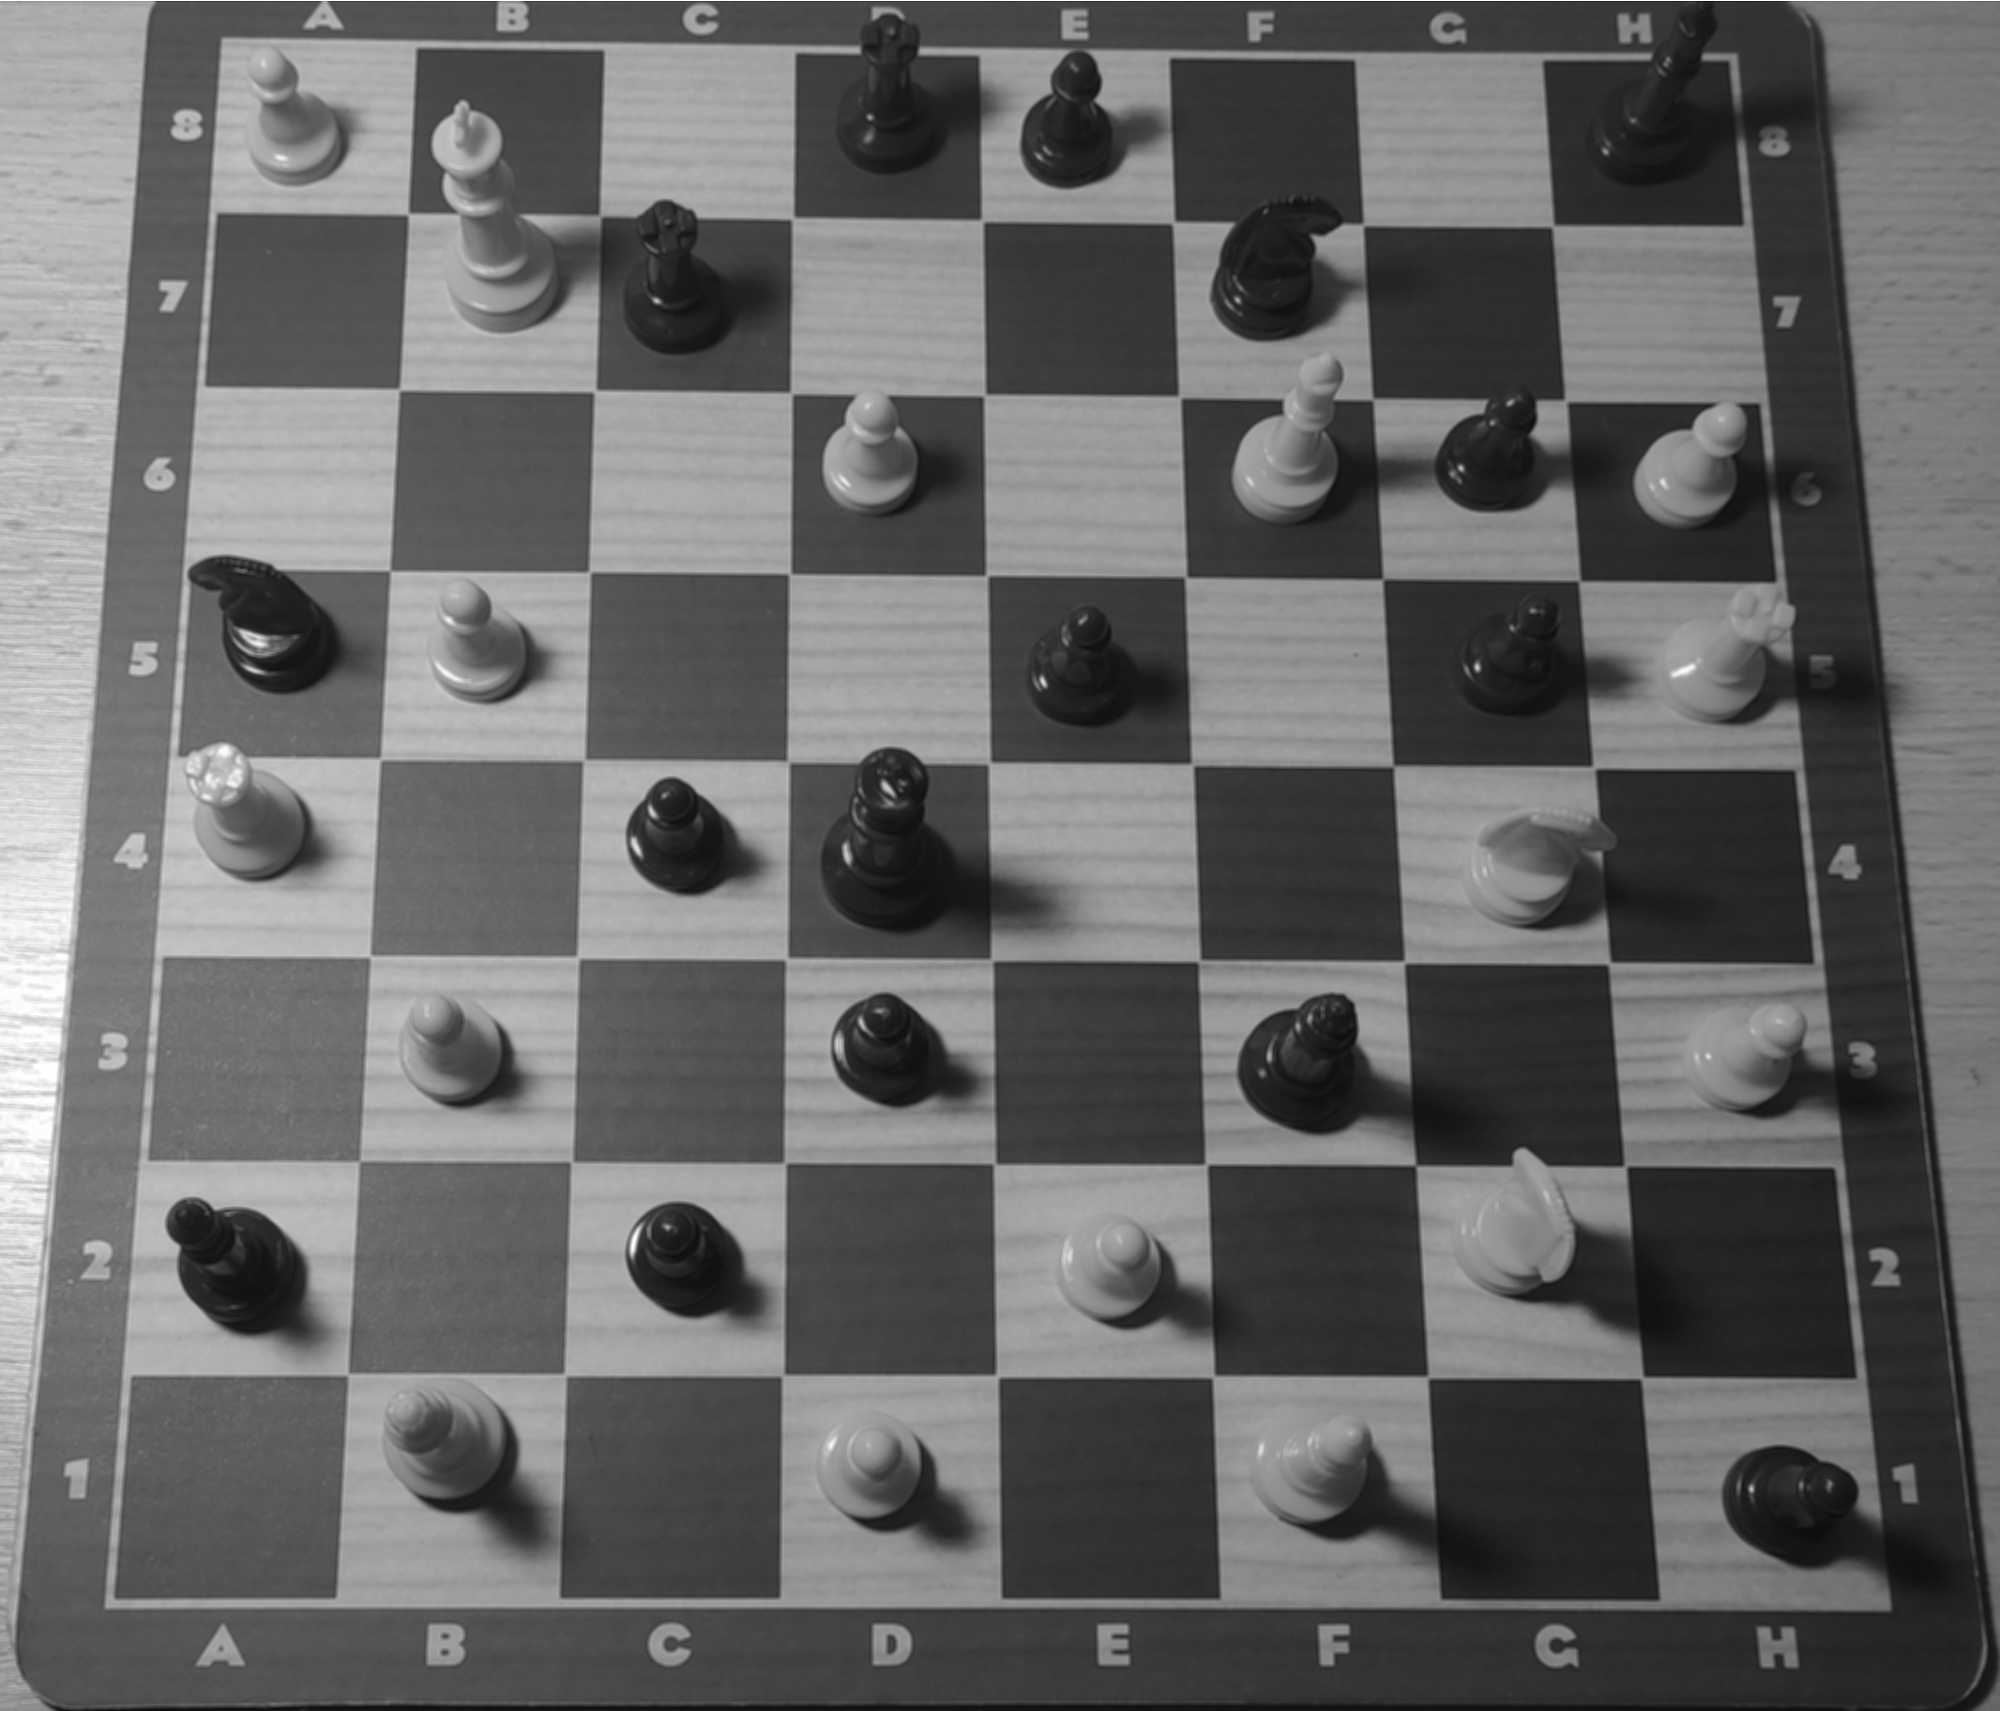
\includegraphics[scale=0.15]{gaussian-blur}
	\caption{Application of the Gaussian blur.}\label{fig:gaussian-blur}
\end{figure}

\subsection{Canny Edge Detection}

Canny edge detection is a technique to extract useful structural information from different vision objects and dramatically reduce the amount of data to be processed. It makes the outlines of objects stand out, which is useful to gather information on the location of the chessboard squares. The values used for the first and second threshold are, respectively, 10.0 and 200.0.

\begin{figure}[H]
	\centering
	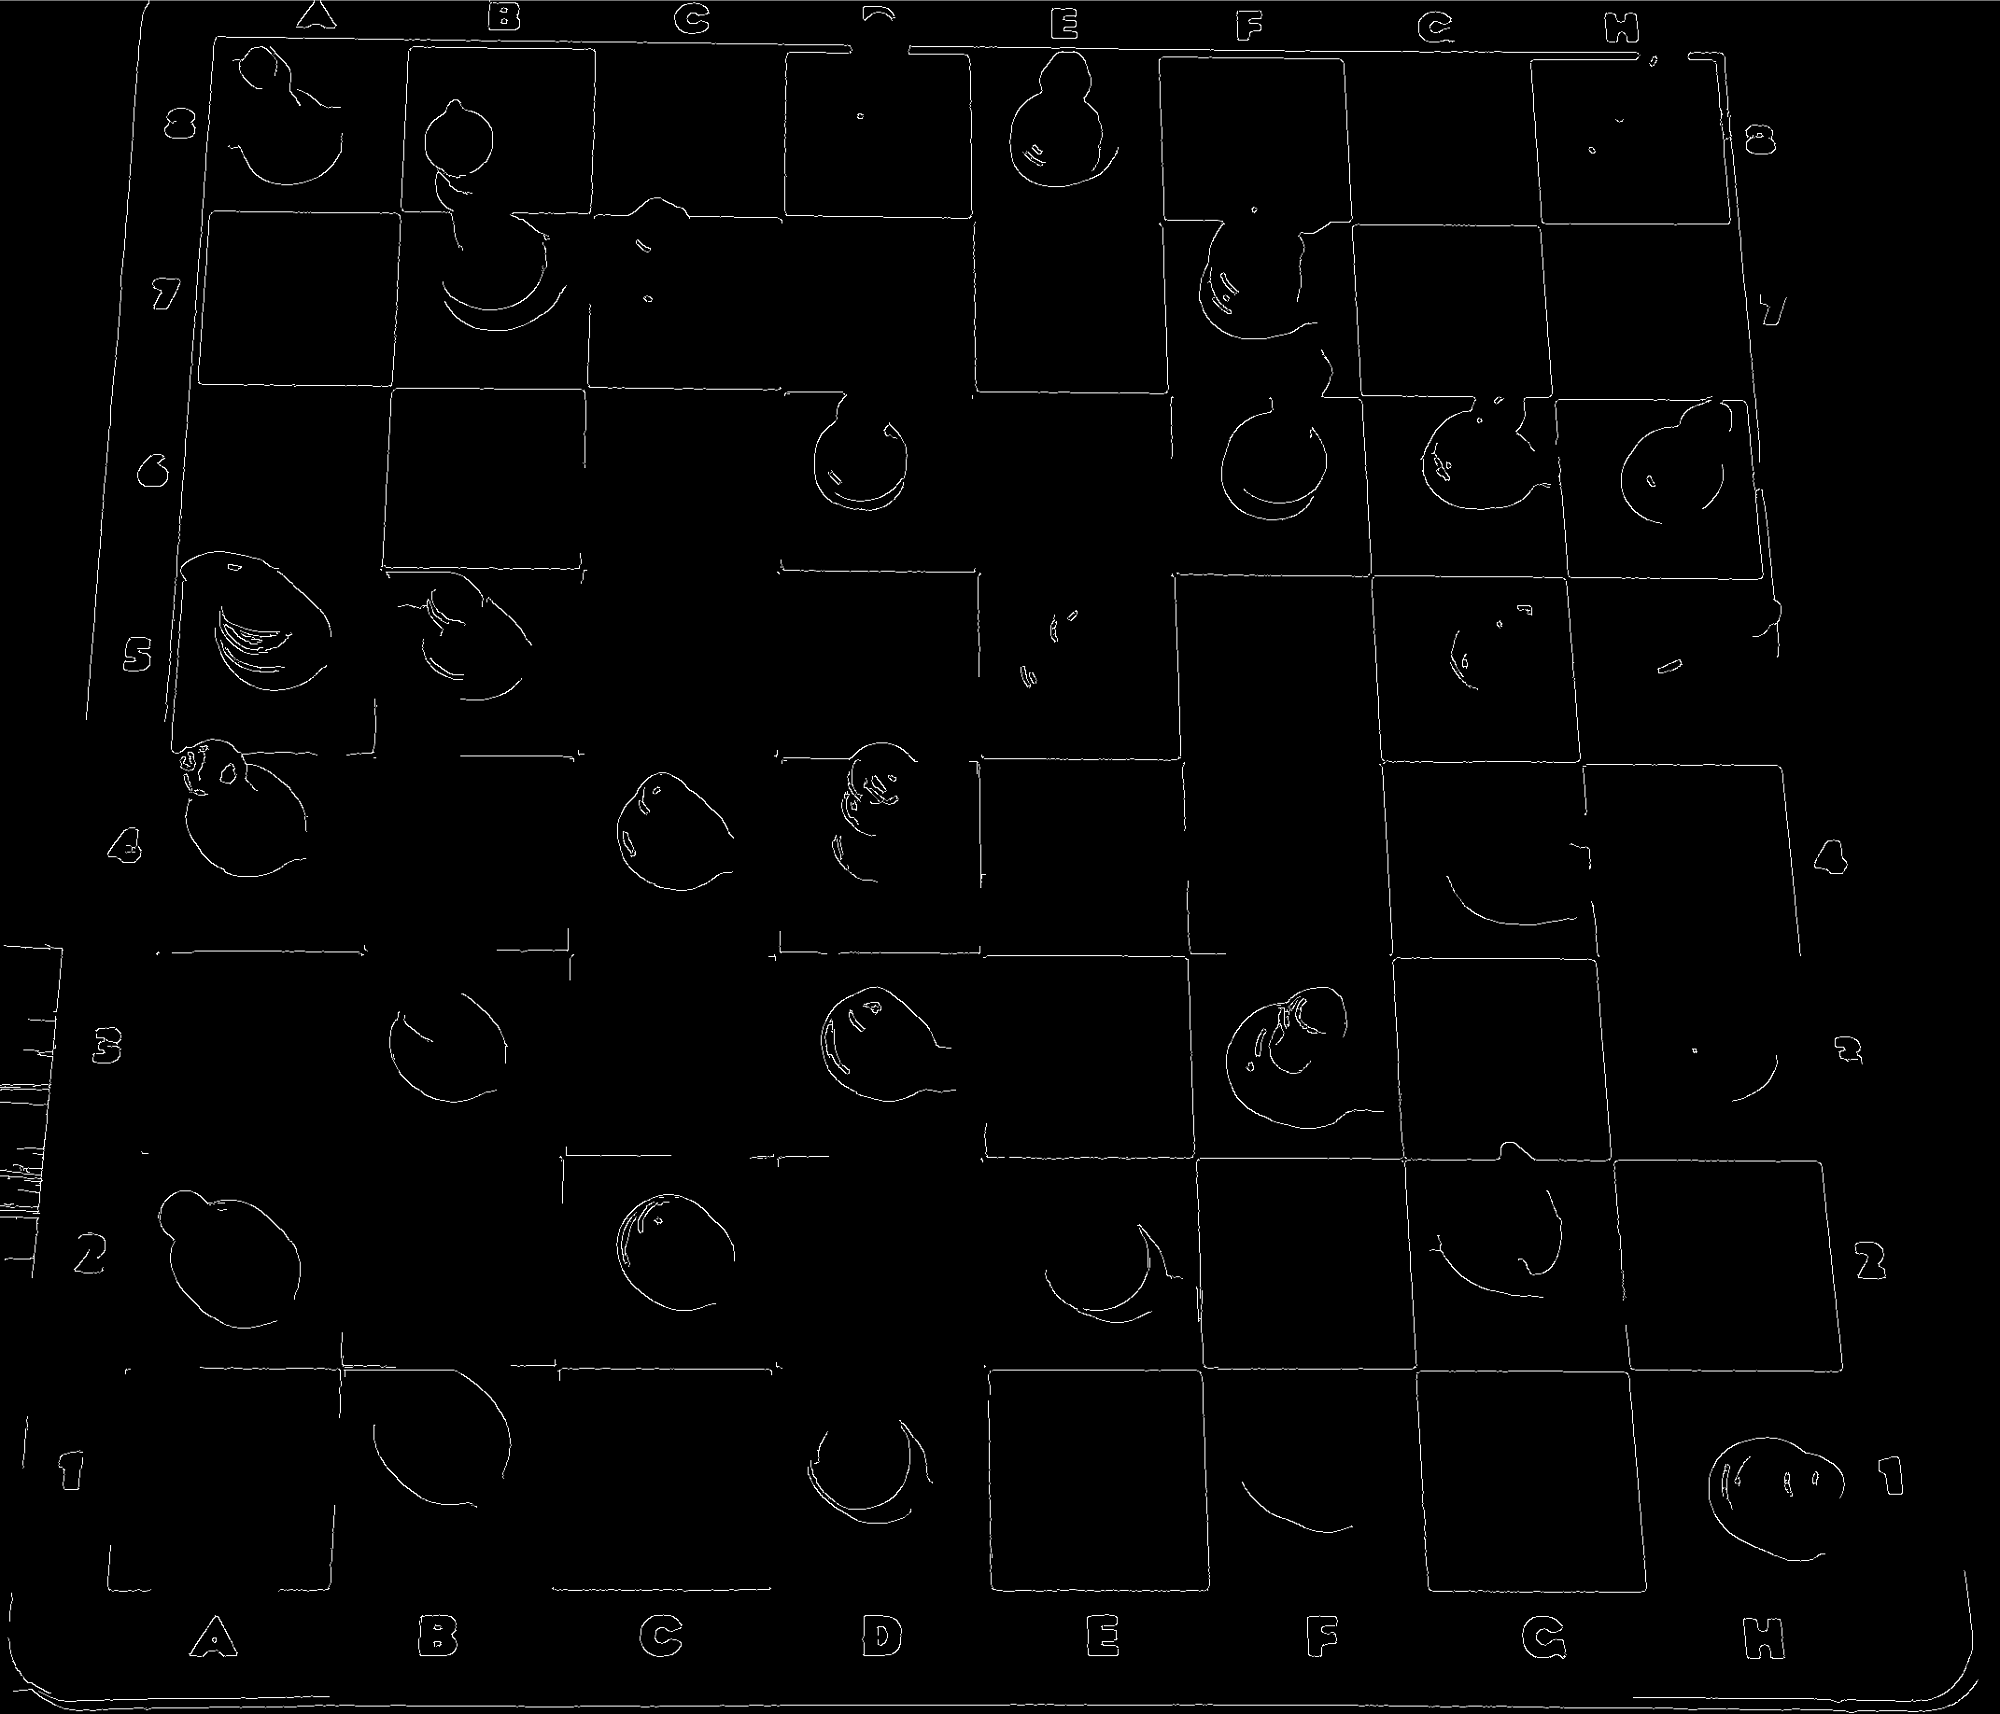
\includegraphics[scale=0.15]{canny-edge}
	\caption{Example application of the Canny Edge detection technique.}\label{fig:canny-edge}
\end{figure}

\subsection{Hough Transform}

The Hough transform is a feature extraction technique, originally concerned with the identification of lines in the image, which is exactly why it is used here: to identify the lines that define the chessboard squares. Applied to the edges made available by the last step's edge detection, we get a rough estimate of all the chessboard lines in the image. The values used for the parameters rho, theta and threshold are, respectively, 1.0, $\frac{\pi}{180}$ and 150.

\begin{figure}[H]
	\centering
	\includegraphics[scale=0.15]{hough}
	\caption{Example application of the Hough Transform.}\label{fig:hough}
\end{figure}

\subsection{Clustering}

In order to remove noise related to the edge detection, k-means is initially used in conjunction with the Hough transform. K-Means clustering is a method of vector quantization, that aims to partition n observations into k clusters in which each observation belongs to the cluster with the nearest mean (cluster centers or cluster centroid), serving as a prototype of the cluster.  . After the k-means clustering is completed, every point in each cluster is averaged out to find the mean point, which is considered as a chessboard square corner.

\begin{figure}[H]
	\centering
	\includegraphics[scale=0.15]{clustering}
	\caption{Example application of K-Means clustering to find the corners (in red) of the squares.}\label{fig:clustering}
\end{figure}

\subsection{Separation into different ROIs}

After all the chessboard square corners have been accounted for, the 64 regions of interest can now be defined. To make sure that all the different possible pieces fit in the ROIs, these are defined with extra width and height, as well as a width and height shift to account for slight picture angle variations.

\begin{figure}[H]
	\centering
	\includegraphics[scale=0.15]{rois}
	\caption{Final ROIs defined with the preprocessing techniques.}\label{fig:rois}
\end{figure}


\section{Convolutional Neural Network}\label{sec:4}

To correctly classify the class a piece belongs to from the different ROIs, a convolutional neural network \cite{1} - short CNN - was used to generate a model. In this case, the CNN is trained and validated using Keras and TensorFlow \cite{2}, and is then converted to TensorFlow Lite so it can run with increased speed on the Android device.

\subsection{Architecture}

Regarding the architecture of the CNN, a sequential \cite{3} model with 10 layers (including output layer) was chosen. The model is then compiled with the Binary Cross-entropy loss function and the Adam optimizer (stochastic gradient descent). The full specification for each layer of the model is represented in the following table. The layer column data is the name of the Keras layer. The Conv2D and Dense layers all use the same (ReLU) activation function, except for the last Dense output layer, which uses the Sigmoid function.

\begin{table}[H]
	\centering
	\begin{tabular}{||c c c c||} 
		\hline
		N & Layer & N Filters/Units & Pool/Kernel Size \\ [0.5ex] 
		\hline\hline
		1 & Conv2D & 32 & 5 x 5\\ 
		\hline
		2 & MaxPooling2D & - & 2 x 2 \\
		\hline
		3 & Conv2D & 64 & 5 x 5 \\
		\hline
		4 & MaxPooling2D & - & 2 x 2 \\
		\hline
		5 & Dropout & - & - \\ [1ex] 
		\hline
		6 & Flatten & - & - \\ [1ex] 
		\hline
		7 & Dense & 128 & - \\ [1ex] 
		\hline
		8 & Dropout & - & - \\ [1ex] 
		\hline
		9 & Dense & 64 & - \\ [1ex] 
		\hline
		10 & Dense & 13 & - \\ [1ex] 
		\hline
	\end{tabular}
	\caption{\label{tab:cnn-architecture}CNN layer architecture.}
\end{table}

\pagebreak

\subsection{Dataset}

The dataset contains all the piece images used for the effect of training and validating the model. It is split into 13 different classes, one for each piece type and color (total of 6*2 = 12) and an empty square class. The used images are three-channel RGB images and are organized into different folders, each being it's own class, and is read directly from it's directory using the Keras utilitary $\textit{image\_dataset\_from\_directory}$ function.

As explained in the Introduction section of this paper, the dataset was partly obtained from similar projects online \cite{4} and partly taken and labeled by myself. It includes different colored chessboards and different shaped pieces and contains around 1130 different images.

\begin{figure}[H]
	\centering
	\begin{minipage}[b]{0.25\textwidth}
		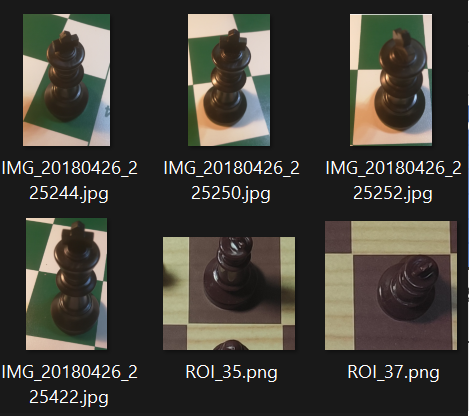
\includegraphics[width=\textwidth]{dataset}
		\caption{Multiple dataset image examples.}
	\end{minipage}
	\hfill
	\begin{minipage}[b]{0.65\textwidth}
		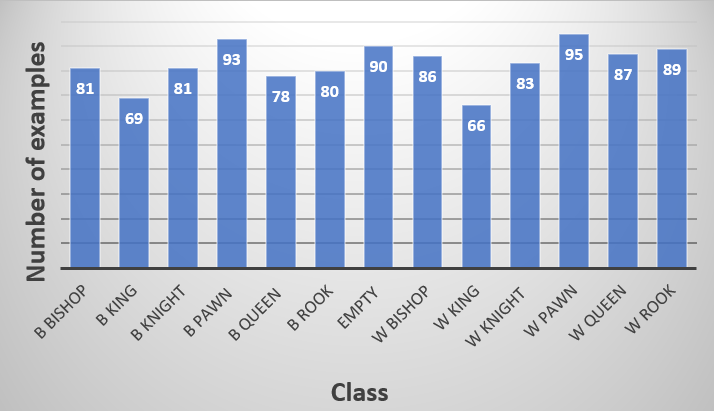
\includegraphics[width=\textwidth]{dataset-count}
		\caption{Image distribution in the dataset.}
	\end{minipage}
\end{figure}


\subsection{Training and Validation}

The CNN was fitted using 80\% of the complete dataset. The other 20\% was used for validation only. The chosen amount of total epochs was 150 and a batch size of 64 was also used.

By the end of the 150th epoch, the training process reported a training loss of 0.0111 and a training accuracy of 0.9889. The validation results were not as good: a validation loss of 0.4156 and a validation accuracy of 0.4622.

\pagebreak

\section{Application}

The proof-of-concept application that ties the preprocessing and usage of the model together was developed exclusively for the Android Operating System. It allows for pictures - either taken in the moment with the camera or loaded from the internal storage - to be run through the preprocessing and the CNN model. The results from this process are then compiled together into an actual virtual chessboard, along with a image of the actual drawn ROIs (for debugging and testing purposes only).

\begin{figure}[H]
	\centering
	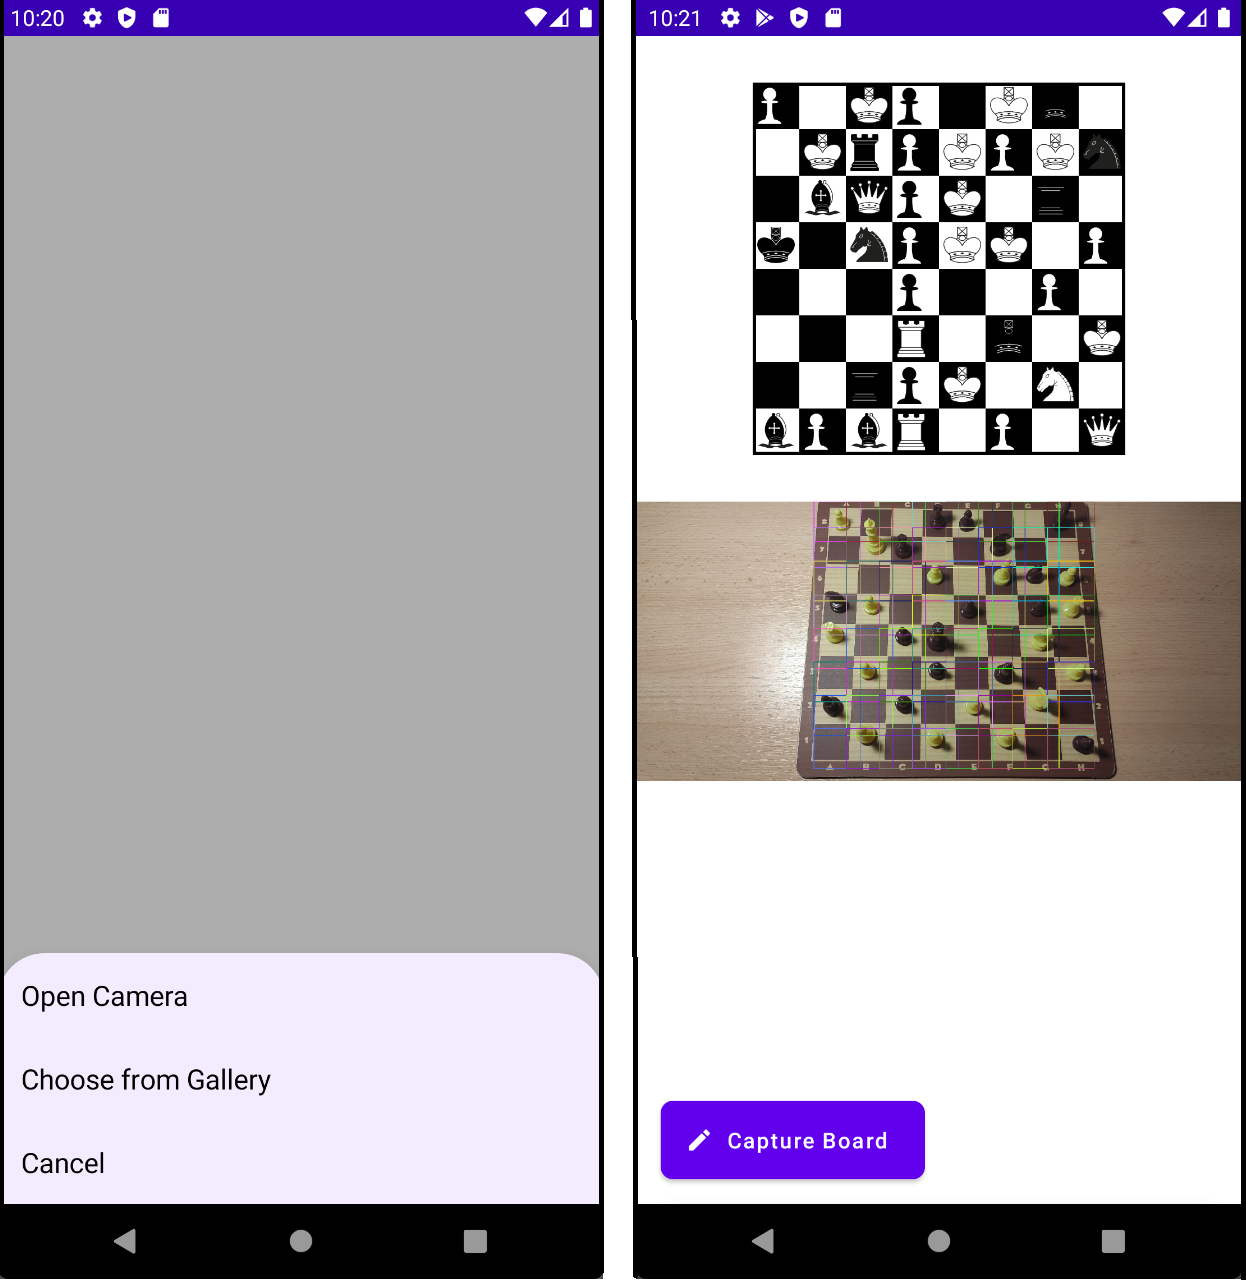
\includegraphics[scale=0.4]{usage}
	\caption{Usage of the application.}\label{fig:usage}
\end{figure}

\pagebreak

\section{Conclusions}\label{sec:5}

Overall, the idea presented in this paper is successful. The image preprocessing showed great results and is near perfect for the needed usage. The proof-of-concept application was also a success, showing that Android - and possibily other mobile operating systems - can run these kind of applications at a good enough speed to be usable on a larger scale.

The biggest problem was the performance of the model, which was not particularly exceptional, leading to less than desired results. This could likely be improved with the usage of a better dataset and a more thorough training and validating process, in general. Still, in the end, the work presented is considered successful because it acts as a good proof-of-concept building foundation for larger projects.

\newpage

\begin{thebibliography}{9}
	\bibitem{1}
	\href{https://en.wikipedia.org/wiki/Convolutional_neural_network}{Wikipedia. Convolutional Neural Network. (Access date: 04.03.2022) [Online]}
	
	\bibitem{2}
	\href{https://viso.ai/edge-ai/tensorflow-lite/}{Viso.ai. TensorFlow-Lite. (Access date: 04.03.2022) [Online]}
	
	\bibitem{3}
	\href{https://keras.io/guides/sequential_model/}{Keras.io. Sequential Model. (Access date: 04.03.2022) [Online]}
	
	\bibitem{4}
	\href{https://towardsdatascience.com/board-game-image-recognition-using-neural-networks-116fc876dafa}{TowardsDataScience. Board Game Image Recognition. (Access date: 04.03.2022) [Online]}
	
	
\end{thebibliography}

\end{document}